\chapter{Related Work}
\label{chap:related-work}
With the rise of computer usage in today's society, they have quite naturally made their way over to education. As such, web-based, computer-based and adaptive assessment systems have been investigated and researched quite thoroughly over the years. The result of this research is numerous tools and software which provide students the opportunity to practise their programming skills, whether it be by writing code or answering programming questions, in an environment which tracks their progress. Almost all of these tools provide the basic features, that is the programming exercises themselves, and a component to view statistics or student results. Some of them distinguish themselves by adding useful and not so common features such as adaptive difficulty. From all the solutions we looked at, very few provided automate exercise generation, and for those who did, their approach was only limited to extremely simple exercises. \newline

We have looked at quite a few solutions such as ELP (Environment for Learning to Program) and CourseMaster, which have the very basic features. We do not go into detail about how these solutions operate since the details are quite straightfowrad and not very interesting. Instead we focus on software which has approached the adaptive difficulty problem, and look into how they did so.\newline

In this section we look at the related software which has influenced the design and implementation of our proposed solution, jSCAPE.

\section{Programming Adaptive Testing}
\label{sec:PAT}
PAT\cite{PAT} is a web-based adaptive testing system, developed in ActionScript/Flash, for assessing students' programming knowledge in Greek high schools. \newline

The assessment is carried out by presenting students with 30 questions from various chapters of the introductory programming course. Some of the questions supported by the PAT system are true/false questions, multiple choice questions, gap filling in a piece of code, questions involving diagrams and questions where one has to determine the behaviour of a piece of code.\newline

In PAT, questions are classified into different difficulty categories. Category A is for easy questions, category B is for intermediate questions and category C is for difficult questions. PAT seeks to adapt the difficulty of the questions to the student's ability, by choosing questions of the appropriate difficulty category.

\begin{figure}[H]
\centering
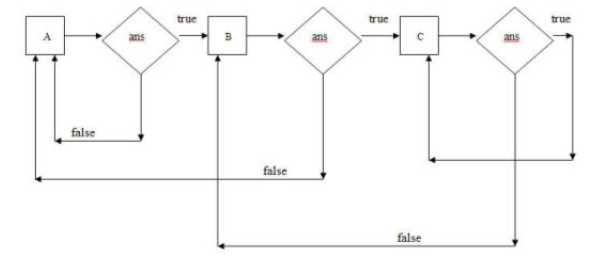
\includegraphics[width=\textwidth,height=\textheight,keepaspectratio]{PAT_adaptive_sequence}
\caption{Adaptive sequence of questions in PAT. (Source:\cite{PAT})}
\label{fig:PAT_adaptive_sequence}
\end{figure}

Figure \ref{fig:PAT_adaptive_sequence} shows the possible adaptive sequences. This algorithm is quite simplistic, every correct answer leads to a promotion to the next level of difficulty until no further promotions are possible. Likewise, every incorrect answer leads to a demotion to a lower level of difficulty until no further demotions are possible.\newline

At the end of the test, the system shows the student's total number of correct answers out of 30 and how well the student performed on each chapter. Also, PAT classifies the student into one of three programming skill levels based on their final score and a weighted score, where the difficulty of the questions answered correctly is considered. These results are available to both students and teachers so that they can be used to improve performance later on in the school year.\newline

We feel that the adaptive algorithm increases the difficulty of questions too quickly and doesn't take into account guessing or possible slip ups from students. This limitation can be circumvented by, for instance, requiring a number of correct answers at the current difficulty level before progressing to the next one.\newline

PAT only provides assessment at specific times throughout the school year and no opportunity for students to practice and self-assess in their own time. In addition, it isn't possible for teachers to upload their own questions to the system. The question bank remains static and contains 443 questions. Lastly, the authors of PAT admit that the statistical data available to students and teachers is fairly limited, and that improvements should be pursued in future work.

\section{SIETTE}
\label{sec:SIETTE}
SIETTE\cite{SIETTE-small} (System of Intelligent Evaluation Using Tests for Tele-education) is a web based environment for generating and constructing adaptive tests. It has been used with great success in courses from the computer science engineering school, the telecommunication engineering school and the philosophy faculty, all at the University of Malaga, Spain.\newline

SIETTE is a vast system, and at the time of publication (2005) it contained information about $15000$ student test sessions, and the knowledge base contained 84 subjects, 1852 topics, 3820 question and 220 tests.\newline

SIETTE is designed to be used by both students and teachers. Teachers use the system to create tests, define the subject topics, the questions and their parameters. Students use the system to take the tests specified by the teachers. The tests can be used for self-assessment, where the correction is shown immediately after the student has answered. Hints and more extensive feedback are also available in this mode. Or, the tests can be used as exams, where the score counts towards the student's final grade. In this mode, hints and feedback aren't provided. It is important to note that tests have a fixed number of questions, thus, new tests must be created every time a student runs out of practice.\newline

As mentioned earlier, SIETTE constructs adaptive tests, therefore, when a student answers a question, his ability is re-estimated and the next question is selected accordingly. Implementation of this is done by using item response theory in the computerized adaptive testing framework.\newline

SIETTE uses the three-parameter logistic (3PL) model and measures the student's knowledge in terms of a discrete random variable $\theta$, which ranges from 0 to $K-1$, where $K$ is the number of discrete knowledge levels. When it comes to creating items, the guessing parameter $c$ is determined automatically, whereas the other two parameters must be entered by the teacher. The discrimination parameter ($a$) must be a number between $0.5$ and $1.5$. The difficulty parameter must be a natural number between 0 and $K-1$. A few years after the SIETTE paper was published, the authors added an item calibration tool because teacher estimates of item parameters are never very accurate.\newline

To estimate students' knowledge level, SIETTE uses the Bayesian estimation method (section \ref{subsec:IRT}) with a knowledge distribution per student, per topic. Also, SIETTE provides teachers with the option of choosing different item selection procedures for tests, such as random selection, difficulty-based selection and bayesian selection.

\begin{figure}[H]
\centering
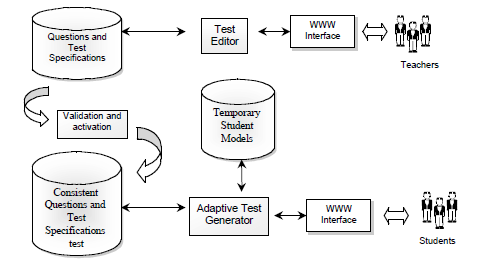
\includegraphics[width=\textwidth,height=\textheight,keepaspectratio]{siette-architecture}
\caption{SIETTE Architecture. (Source:\cite{SIETTE})}
\label{fig:siette-architecture}
\end{figure}

Figure \ref{fig:siette-architecture} gives on overview of the SIETTE architecture. The system is comprised of several components\cite{SIETTE-components}:
\begin{itemize}
\item The \textit{knowledge base}: where tests, topics and questions are stored. Some supported question types are true/false, multiple choice, multiple response and fill-in-the-gap. More interactive questions also exist, implemented as Java applets, where one has to color parts of a map, or move around objects so that they appear chronologically, for example.
\item The \textit{student model repository}: a collection of student models, where information about students' knowledge level estimation, which questions they answered, etc... is stored.
\item The \textit{student workspace}: a web interface where students take tests.
\item The \textit{test editor}: a tool where teachers can define tests, topics, questions.
\item The \textit{result analyzer}: a tool which presents graphical data about students' performance, knowledge estimation levels, etc...
\item The \textit{item calibration tool}: a module used to calibrate items by determining the item parameters (difficulty, discrimination and pseudo-chance).
\end{itemize}

SIETTE is a large and complex system, containing many useful features relevant to the area of web-education, and going through all of these wouldn't be possible. Since SIETTE has been used to such success in university courses we decide to inspire ourselves from this system, especially for the implementation of the adaptive difficulty component. Details about the algorithms used in SIETTE, and hence jSCAPE, can be found in section \ref{sec:implementing-cat}, with Java code to illustrate. However, SIETTE does not provide mechanisms to automatically generate exercises, and so we shall define our own algorithms for this.

\section{Summary}
We have looked at some of the relevant work in the field of computer based education and assessment. We saw that PAT provided a simple algorithm for increasing or decreasing the difficulty of exercises, and so an improved version of this algorithm will feature in jSCAPE. We also saw that SIETTE provided many of the features we set out to replicate in jSCAPE, therefore particular parts of our implementation will be inspired by SIETTE.\newline

SIETTE is the most complete system we have come across while doing research for this project. Moreover, examining some existing solutions which haven't been detailed in this section, has given us insight into the most common features available in these types of systems. \newline

In the next chapter we present the system developed as part of this project: jSCAPE. 